\documentclass{sig-alternate}
%DIF LATEXDIFF DIFFERENCE FILE
%DIF DEL Draft7.tex                        Tue Oct 25 01:18:29 2016
%DIF ADD AligningWordSenseEmbeddings.tex   Tue Oct 25 00:59:07 2016
%DIF 2c2
%DIF < \usepackage[dvipsnames]{xcolor}
%DIF -------
 %DIF > 
%DIF -------
%\documentclass{article}
%DIF 4c4
%DIF < \usepackage[subpreambles=true]{standalone}
%DIF -------
\usepackage[subpreambles=false]{standalone} %DIF > 
%DIF -------


\usepackage{csquotes}
\usepackage{amsmath}
%DIF 9a9-16
 %DIF > 
\usepackage[all=normal, %DIF > 
paragraphs=tight, %DIF > 
floats=tight, %DIF > 
%mathspacing=tight, %DIF > 
%wordspacing=tight, %DIF > 
tracking=tight, %DIF > 
bibbreaks=tight]{savetrees} %DIF > 
%DIF -------
\usepackage{microtype}
\usepackage{adjustbox}

 %\usepackage[subpreambles=true]{standalone}
\usepackage{environ}
\RenewEnviron{adjustbox}{Nothing here}


%DIF 11a19
\usepackage{flushend} %DIF > 
%DIF -------

\usepackage{booktabs, array} % Generates table from .csv
\usepackage{pgfplots, pgfplotstable}

%DIF 15a24
 %DIF > 
%DIF -------
\pgfplotsset{
compat=1.12,
/pgfplots/table/search path={.,..,../data}
}

%DIF 20a30-32
%\usepackage[dvipsnames]{xcolor} %DIF > 
\usepackage{tikz} %DIF > 
\usetikzlibrary{positioning}
\usetikzlibrary{shapes} 
\usetikzlibrary{arrows.meta}
\usetikzlibrary{decorations.pathmorphing}


\tikzset{
	tripleinner/.style args={[#1] in [#2] in [#3]}{
		#1,preaction={preaction={draw,#3},draw,#2}
	},
	triple/.style={%
		tripleinner={[line width=0.5pt,black] in
			[line width=3pt,white] in
			[line width=4pt,black]}	 
	}
}

\tikzset{
	input/.style={
		%circle,
		%draw,
		%Blue,
		minimum width = 2
	},
	datastore/.style={cylinder,
		draw,
		%Green,
		minimum width = 2
	},
	proc/.style={rectangle,
		draw,
		%Red,
		minimum size = 50
	},
	link/.style={->,
		black},
	multi/.style={-Implies,
		triple,
	},
	labe/.style={
		%Blue,
		fill=white,
		fill opacity=0.6,
		text opacity=1,
		font={\footnotesize\itshape}	
	}
} %DIF > 
%DIF -------

%DIF 21a34
 %DIF > 
%DIF -------
\usepackage[backend=bibtex,
%DIF 22-23c36-38
%DIF < style=trad-abbrv,url=false, doi=false,
%DIF < sorting=none, sortcites=true]{biblatex}
%DIF -------
style=ieee,url=false, doi=false, isbn=false, %DIF > 
sorting=none, sortcites=true, hyperref=false]{biblatex} %DIF > 
 %DIF > 
%DIF -------
\bibliography{master}

\usepackage[author={Lyndon White}]{pdfcomment}
\usepackage{cleveref}

\newcommand{\W}{\mathcal{W}}
\renewcommand{\c}{\mathbf{c}}
\newcommand{\s}{\mathbf{s}}
\renewcommand{\l}{\mathbf{l}}
\renewcommand{\u}{\mathbf{u}}
\newcommand{\ci}{\perp\!\!\!\perp} % from Wikipedia
\DeclareMathOperator*{\argmin}{arg\,min}
\DeclareMathOperator*{\argmax}{arg\,max}
 %DIF > 
\newcommand{\wordquote}[1]{\enquote{\texttt{#1}}} %DIF > 
%DIF PREAMBLE EXTENSION ADDED BY LATEXDIFF
%DIF UNDERLINE PREAMBLE %DIF PREAMBLE
\RequirePackage[normalem]{ulem} %DIF PREAMBLE
\RequirePackage{color}\definecolor{RED}{rgb}{1,0,0}\definecolor{BLUE}{rgb}{0,0,1} %DIF PREAMBLE
\providecommand{\DIFadd}[1]{{\protect\color{blue}\uwave{#1}}} %DIF PREAMBLE
\providecommand{\DIFdel}[1]{{\protect\color{red}\sout{#1}}}                      %DIF PREAMBLE
%DIF SAFE PREAMBLE %DIF PREAMBLE
\providecommand{\DIFaddbegin}{} %DIF PREAMBLE
\providecommand{\DIFaddend}{} %DIF PREAMBLE
\providecommand{\DIFdelbegin}{} %DIF PREAMBLE
\providecommand{\DIFdelend}{} %DIF PREAMBLE
%DIF FLOATSAFE PREAMBLE %DIF PREAMBLE
\providecommand{\DIFaddFL}[1]{\DIFadd{#1}} %DIF PREAMBLE
\providecommand{\DIFdelFL}[1]{\DIFdel{#1}} %DIF PREAMBLE
\providecommand{\DIFaddbeginFL}{} %DIF PREAMBLE
\providecommand{\DIFaddendFL}{} %DIF PREAMBLE
\providecommand{\DIFdelbeginFL}{} %DIF PREAMBLE
\providecommand{\DIFdelendFL}{} %DIF PREAMBLE
%DIF END PREAMBLE EXTENSION ADDED BY LATEXDIFF

\begin{document}

\title{Finding Word Sense Embeddings Of Known Meaning}

\DIFaddbegin \numberofauthors{4}
\author{
	\alignauthor \DIFadd{Lyndon White}\\
	%DIF > \affaddr{School of Electrical, Electronic and Computer Engineering}\\
	\affaddr{University of Western Australia}\\
	\email{lyndon.white@research.uwa.edu.au}
	%DIF > 
	\alignauthor \DIFadd{Roberto Togneri}\\
	%DIF > \affaddr{School of Electrical, Electronic and Computer Engineering}\\
	\affaddr{University of Western Australia}\\
	\email{roberto.togneri@uwa.edu.au}
	%DIF > 
	\alignauthor \DIFadd{Wei Liu}\\
	%DIF > \affaddr{School of Computer Science and Software Engineering}\\
	\affaddr{University of Western Australia}\\
	\email{wei.liu@uwa.edu.au}
	%DIF > 
	\and
	%DIF > 
	\alignauthor \DIFadd{Mohammed Bennamoun}\\
	%DIF > \affaddr{School of Computer Science and Software Engineering}\\
	\affaddr{University of Western Australia}\\
	\email{mohammed.bennamoun@uwa.edu.au}
} 
%DIF > There are instructions about shared affilations on https://www.acm.org/sigs/publications/sigfaq#a17

\DIFaddend \maketitle





\begin{abstract}
Word sense embeddings are vector representations of polysemous words -- words with multiple meanings. Similar techniques to those used to find word embedding vectors, such as in Word2Vec, are often used to learn multiple sense embeddings for each word.
These induced sense embeddings, however, do not necessarily correspond to any dictionary senses of the word.
This limits the applicability of these embeddings in traditional semantic-orientated tasks such as lexical word sense disambiguation.
To overcome this, we propose a method to find new sense embeddings of known meaning.
We term this method refitting, as the new embedding is fitted to model the meaning of a target word in the example sentence. The refitting is accomplished using probabilities of the existing induced sense embeddings, as well as their vector values.

Our contributions are threefold:
\DIFaddbegin \DIFadd{(1) }\DIFaddend The refitting method to find the new sense embeddings;
 \DIFaddbegin \DIFadd{(2) }\DIFaddend a novel smoothing technique, for use with the refitting method;
and \DIFaddbegin \DIFadd{(3) }\DIFaddend a new similarity measure for words in context, \DIFaddbegin \DIFadd{defined by }\DIFaddend using these refitted sense embeddings.

We show how our refitting based techniques improve the performance of the Adaptive Skip-Gram sense embeddings for word similarly evaluation; and how it allows the embeddings to be used for lexical word sense disambiguation -- which was not possible before refitting the sense embeddings.
Further to this, the similarity measure we derive from the refitting has significantly better time-complexity than the commonly used AvgSimC; making this more a more suitable method for large scale web-scale datasets.
\end{abstract}


\section{Introduction}


\DIFdelbegin \DIFdel{Word embeddings }\DIFdelend \DIFaddbegin \DIFadd{Popular word embedding vectors, such as Word2Vec }\parencite{mikolov2013efficient} \DIFadd{and GLoVE }\parencite{pennington2014glove}\DIFadd{, }\DIFaddend represent a word's semantic meaning and \DIFaddbegin \DIFadd{its }\DIFaddend syntactic role as a point in a vector space\DIFdelbegin %DIFDELCMD < \parencite{NPLM, collobert2008unified, mikolov2013efficient}%%%
\DIFdel{. However, }\DIFdelend \DIFaddbegin \DIFadd{. As }\DIFaddend each word is only given one embedding \DIFdelbegin \DIFdel{-- which restricts it to representing only one combined sense. Word sense embeddings }\DIFdelend \DIFaddbegin \DIFadd{such method are restricted to only representing a single combined sense, or meaning, of the word. }\emph{\DIFadd{Word sense embeddings}} \DIFaddend are the generalisation of \DIFdelbegin \DIFdel{this }\DIFdelend \DIFaddbegin \DIFadd{word embeddings }\DIFaddend to handle polysemous and homonymous  words. Often these \DIFdelbegin \DIFdel{word }\DIFdelend sense embeddings are learnt through unsupervised word sense induction \parencite{Reisinger2010,Huang2012,tian2014probabilistic, AdaGrams}. \DIFdelbegin \DIFdel{In these cases it is not possible to directly determine which meaning belongs to which embedding. Furthermore the induced senses }\DIFdelend \DIFaddbegin \DIFadd{The induced sense embeddings }\DIFaddend are unlikely to directly \DIFdelbegin \DIFdel{match to any one }\DIFdelend \DIFaddbegin \DIFadd{coincide with any set of }\DIFaddend human defined meaning at all\DIFdelbegin \DIFdel{; but rather will }\DIFdelend \DIFaddbegin \DIFadd{, i.e. they will not match lexical senses such as those defined in a lexical dictionary, eg WordNet }\parencite{miller1995wordnet}\DIFadd{. These induced senses can }\DIFaddend be more specific, more broad, or include the meanings of jargon not in common use.


It can be argued that many word sense induction (WSI) systems may capture better \DIFaddbegin \DIFadd{word }\DIFaddend senses than human lexicographers \DIFaddbegin \DIFadd{do manually}\DIFaddend , however this does not mean that induced senses can replace standard lexical senses. While the induced senses may cover the space of meanings more comprehensively, or with better granularity than the \DIFdelbegin \DIFdel{standard senses, there is a }\DIFdelend \DIFaddbegin \DIFadd{lexical senses, it is important to appreciate the }\DIFaddend vast wealth of existing knowledge defined around lexical senses from various sense inventories. Methods to link induced senses to lexical senses allow \DIFdelbegin \DIFdel{this information to be unlocked}\DIFdelend \DIFaddbegin \DIFadd{us to take advantage of both worlds}\DIFaddend .


\DIFdelbegin \DIFdel{We thus propose a method for using a single example of a word in context to synthesise a new embedding for that particular sense.
We term this }\emph{\DIFdel{refitting}} %DIFAUXCMD
\DIFdel{the induced senses, as it combines them to fit to the meaning in }\DIFdelend \DIFaddbegin \DIFadd{In this paper, we propose a refitting method to generate a sense embedding vector that matches with a labelled lexical sense.
Given an example sentence with the labelled lexical sense of a particular word, }\DIFaddend the \DIFdelbegin \DIFdel{example sentence}\DIFdelend \DIFaddbegin \DIFadd{refitting method algorithmically combined the induced sense embeddings of the target word in a way such that the likelihood of the example sentence, is similar usages, is maximised.
With the refitting, the induced sense embeddings are not restrict ot be used only in the system they are obtained from, but can also be used in more general situations where standard senses, or user defined senses are desired}\DIFaddend .
\DIFdelbegin \DIFdel{Our method allows us to use a single labelled example to produce a labelled sense embedding. This allows a shift from a representation that can only work within the system , to one that uses a standard sense, or a user defined sense, which can be used as part of a more complex knowledge engineering system. 
}\DIFdelend 


Refitting word sense vectors to match a lexicographical sense inventory, such as WordNet or a translator's dictionary, is possible if the sense inventory features at least one example of the target senses use. The new lexically refitted sense embedding can then be used for Word Sense Disambiguation (WSD). 
Applying WSD \DIFdelbegin \DIFdel{adds useful information to a unstructured document , allowing further processing methods to take advantage of this information.
An application of this would be as part of }\DIFdelend \DIFaddbegin \DIFadd{is almost indispensable in any unstructured document understanding.
For example, }\DIFaddend a machine translation system\DIFdelbegin \DIFdel{. To }\DIFdelend \DIFaddbegin \DIFadd{: to }\DIFaddend properly translate a word, the correct sense should be determined, as different senses in the source language, often translate to entirely different words in the target language.
\DIFdelbegin \DIFdel{Using WSD to add sense annotation to a document bridges between unstructured raw text data to sense annotated data allowing for further processing with systems that require this structure. The application of our method for WSD is discussed }\DIFdelend \DIFaddbegin \DIFadd{We demonstrate how the refitting method can be successfully applied for WSD }\DIFaddend in \Cref{lexicalWSD}.

Beyond refitting to a standard lexical sense, refitting to a user provided example has applications in information retrieval. Consider the natural language query \DIFdelbegin %DIFDELCMD < \enquote{Find me all webpages about banks as in \enquote{the river banks were very muddy.}}%%%
\DIFdelend \DIFaddbegin \wordquote{Find me web-pages about banks as in \enquote{the river banks were very muddy.}}\DIFaddend . By generating an embedding vector for that specific sense of ``banks'' from the example sentence, and \DIFdelbegin \DIFdel{generating }\DIFdelend \DIFaddbegin \DIFadd{by comparing with the generated }\DIFaddend one from use of the \DIFaddbegin \DIFadd{same }\DIFaddend word in each retrieved document, we can \DIFdelbegin \DIFdel{approximate measuring }\DIFdelend \DIFaddbegin \DIFadd{more accurately measure their }\DIFaddend distance in a semantic space. This allows for similarity ranking -- discarding irrelevant uses of the word. The method we propose, using our refitted embeddings, has lower time complexity than AvgSimC \DIFaddbegin \parencite{Reisinger2010}\DIFaddend , the current state of the art alternative for measuring similarity of words in context. This is detailed in \Cref{RefittedSimVsAvgSimC}\DIFaddbegin \DIFadd{.
}\DIFaddend 



\DIFdelbegin \DIFdel{Our refitting method synthesises a new sense vector using the existing induced word sense vectors and the language model.
The new vector is formed as an appropriately weighted sum of the original embeddings. A weighting of the induced sense vectors is determined using the language model and the example sentence.
The refitted vector approximately corresponds to the meaning given by the example sentence. 
Our refitting method is detailed in \mbox{%DIFAUXCMD
\Cref{refitting}}%DIFAUXCMD
.
}%DIFDELCMD < 

%DIFDELCMD < \pdfcomment{How can I (should I?) rewrite the ``We noted that while our refitted'' sentence to not be in past tense}
%DIFDELCMD < %%%
\DIFdel{We noted that while our refitted sense vectors did capture the meaning of the example sentence, }\DIFdelend \DIFaddbegin \DIFadd{We noted during refitting }\DIFaddend often a single induced sense would dominate the refitted sense representation. It is rare in natural language for the meaning to be so \DIFdelbegin \DIFdel{clearly cut}\DIFdelend \DIFaddbegin \DIFadd{unequivocal}\DIFaddend . Generally, a significant overlap exists between the meaning of different lexical senses, and there is often a high level of disagreement when humans are asked to annotate a corpus \parencite{veronis1998study}. We thus would expect \DIFdelbegin \DIFdel{this also to be true when }\DIFdelend \DIFaddbegin \DIFadd{similar to hold }\DIFaddend automatically determining the appropriateness of the induced senses, as is done during refitting. Towards this end, we develop a smoothing method, which we call \emph{geometric smoothing} that de-emphasises the sharp decisions made by the (unsmoothed) refitting method. We found that this significantly improves \DIFaddbegin \DIFadd{the }\DIFaddend results. This suggests that the sharpness of decisions from the language model \DIFdelbegin \DIFdel{may be an artefact of the training method and the sparseness of the training data}\DIFdelend \DIFaddbegin \DIFadd{is an issue with the language model}\DIFaddend , which smoothing can correct. The geometric smoothing method is presented in \Cref{smoothing}.


We demonstrate the refitting method on \DIFaddbegin \DIFadd{sense embedding vectors induced using }\DIFaddend Adaptive Skip-Grams (AdaGram) \parencite{AdaGrams}, \DIFdelbegin \DIFdel{and on our }\DIFdelend \DIFaddbegin \DIFadd{as well as }\DIFaddend own simple greedy word sense embeddings. The method is \DIFdelbegin \DIFdel{generally }\DIFdelend applicable to any skip-gram-like language model that can take a sense vector as its input, and can output the probability of a word appearing in that sense's context.


The rest of the paper is organised as follows: \Cref{relatedwords} discusses \DIFdelbegin \DIFdel{related works on }\DIFdelend \DIFaddbegin \DIFadd{two camps of related works, one on directly }\DIFaddend learning standard lexical sense repressions\DIFdelbegin \DIFdel{directly, and on associating the }\DIFdelend \DIFaddbegin \DIFadd{, and the other on on indirectly associating }\DIFaddend induced senses with standard lexical senses. \Cref{Framework} presents our refitting method, as well as the geometric smoothing method used with it. \Cref{lexicalWSD} shows how the refitted sense vectors can be used for lexical word sense disambiguation. \Cref{SimilarityInContext} describes the RefittedSim measure for word similarity in context, and presents its results. Finally, the paper \DIFdelbegin \DIFdel{presents it's conclusions }\DIFdelend \DIFaddbegin \DIFadd{concludes with outlook to future works }\DIFaddend in \Cref{conclusion}.

\section{Related Works} \label{relatedwords}

\subsection{Directly Learning Lexical Sense Embeddings}
\DIFdelbegin \DIFdel{Our refitting method can be considered as learning lexical sense embeddings , as a one-shot learning task. A alternative is to transform the problem into a supervised}\DIFdelend \DIFaddbegin \DIFadd{In this camp of research, the induction of word sense embeddings is treated as a supervised, }\DIFaddend or semi-supervised \DIFdelbegin \DIFdel{learning task. The difficulty lies in how to get a sufficient number of labelled senses.
One option is to use a separate WSD method to artificially label an unlabelled corpus.
}\DIFdelend \DIFaddbegin \DIFadd{task, that requires sense labelled corpora for training.
}\DIFaddend 

Iacobacci et al. \parencite{iacobacci2015sensembed} use a Continuous Bag of Word \DIFdelbegin \DIFdel{(CBOW)  }\DIFdelend language model \parencite{mikolov2013efficient}, \DIFdelbegin \DIFdel{but use }\DIFdelend \DIFaddbegin \DIFadd{using }\DIFaddend word senses as the labels rather than words. This is a direct application of word embedding techniques. To overcome the lack of a large sense labelled corpus, Iacobacci et al. use \DIFdelbegin \DIFdel{the }\DIFdelend \DIFaddbegin \DIFadd{a }\DIFaddend 3rd party WSD tool\DIFaddbegin \DIFadd{, }\DIFaddend BabelFly, to add sense annotations to a previously unlabelled corpus.
\DIFdelbegin \DIFdel{An alternative approach would be to use a method that disambiguates the senses using a partially trained model.
}\DIFdelend 

Chen et al. \DIFaddbegin \parencite{Chen2014} \DIFaddend use a semi-supervised approach to train sense vectors\DIFdelbegin %DIFDELCMD < \parencite{Chen2014}%%%
\DIFdelend . They partially disambiguate their training corpus, using \DIFdelbegin \DIFdel{their }\DIFdelend initial word sense vectors and WordNet; and use these labels to fine-turn their embeddings.
Initially the sense vectors are set as the average of the single sense word embeddings \parencite{mikolov2013efficient} for the words in the WordNet gloss.
Similarly, \DIFdelbegin \DIFdel{they define }\DIFdelend a context vector \DIFdelbegin \DIFdel{, }\DIFdelend \DIFaddbegin \DIFadd{is defined }\DIFaddend as the average of all words in a sentence.
They then progressively label the words with the sense \DIFdelbegin \DIFdel{of the sense }\DIFdelend vector that is closest to the context vector if it is closer than a \DIFdelbegin \DIFdel{fixed }\DIFdelend \DIFaddbegin \DIFadd{predefined }\DIFaddend threshold.
The requirement for meeting a threshold in order to add the sense label  decreases the likelihood of training on an incorrect sense label.
The selected sense vector is used to update the context vector and then the next word is relabelled. They give two methods for selecting the order of relabelling.
After the relabelling is complete they fine tune the sense embeddings by defining a new skip-gram method with the objective of predicting both the words and the word senses in the context, when given \DIFdelbegin \DIFdel{a }\DIFdelend \DIFaddbegin \DIFadd{an }\DIFaddend input word\footnote{Note that using the input word to predict the which word senses will appear in the context is the opposite of the approach used by AdaGram. AdaGram uses the word sense to predict the word of the context \parencite{AdaGrams}.}. The overall approach is to use the initial sense vectors estimated from the glosses to add sense labels to some of the words, and then use these as the training target.


\DIFaddbegin \DIFadd{Our refitting method learns a new sense embedding as a weighted sum of existing induced sense embeddings of the target word.
This is analogous to regression learning or one-shot learning using refitting.
}\DIFaddend The key practical difference between the one-shot approach used by refitting, compared to the supervised, and semi-supervised approach uses in existing works is the time taken to  add a new sense.
\DIFdelbegin \DIFdel{With our refitting fitting approach adding }\DIFdelend \DIFaddbegin \DIFadd{Adding }\DIFaddend a new sense \DIFaddbegin \DIFadd{using our approach }\DIFaddend is practically instantiations, and replacing the entire sense inventory\DIFaddbegin \DIFadd{, of several hundred thousand senses, }\DIFaddend is only a matter of a few hours.
Whereas for the existing approaches adding senses would require almost fully repeating the training process, often taking several days.
Refitting is a process done to sense word embeddings, rather a method for finding sense embeddings from a large corpus. 
It can be applied to any pretrained sense embeddings, so long as it \DIFdelbegin \DIFdel{meets the requirement for a suitable language model }\DIFdelend \DIFaddbegin \DIFadd{uses a language model based approach}\DIFaddend .
\pdfcomment{Should I mention that it could be adapted to apply to both the embeddings above, with some adaption?}



\DIFdelbegin \DIFdel{One of the key reasons, that it is useful to have senses that align with standard lexical senses , is that it allows word sense embeddings to be used for word sense disambiguation. This is demonstrated by Chen et al.  }%DIFDELCMD < \parencite{Chen2014}%%%
\DIFdel{, and we discuss how refitted word sense vectors can be used do the same in \mbox{%DIFAUXCMD
\Cref{eq:lexicalwsd}}%DIFAUXCMD
. If the word senses do not correspond to the lexical senses, then one approach }\DIFdelend \DIFaddbegin \subsection{Mapping induced senses to lexical senses}\label{mapping}
\DIFadd{Rather than learning lexical senses directly, and alternative camp of thought }\DIFaddend is to form a weighted mapping from induced senses, to the lexical senses.
 \DIFdelbegin %DIFDELCMD < 

%DIFDELCMD < \subsection{Mapping induced senses to lexical senses}%DIFDELCMD < \label{mapping}%%%
%DIFDELCMD <  %%%
\DIFdelend Agirre et al. \DIFaddbegin \parencite{agirre2006} \DIFaddend give a general method to allow induced word senses to be used for lexical WSD\DIFdelbegin %DIFDELCMD < \parencite{agirre2006}%%%
\DIFdelend .
Their method applies to all word sense induction systems, not just word embedding systems, so is more general than the refitting approach that we present.
Their method maps the induced sense disambiguation scores, to scores for disambiguating standard lexical senses. This method was used for \DIFdelbegin \DIFdel{the }\DIFdelend SemEval-2007 Task 02 \parencite{SemEval2007WSIandWSD} to evaluate all entries.
They use an annotated \emph{mapping corpus} to construct a mapping weight between induced senses probabilities and the lexical sense probabilities.

For \DIFdelbegin \DIFdel{$\l=\{l_1,...\}$ }\DIFdelend \DIFaddbegin \DIFadd{$\l=\{l_1,..., l_m\}$ }\DIFaddend the set of lexically defined senses, \DIFdelbegin \DIFdel{$\u=\{u_1,...\}$ }\DIFdelend \DIFaddbegin \DIFadd{$\u=\{u_1,...,u_n\}$ }\DIFaddend the set of unsupervised induced senses, and a corpus of labelled contexts \DIFdelbegin \DIFdel{$\{\c_1, ...\}$ }\DIFdelend \DIFaddbegin \DIFadd{$\{\c_1, ...,c_k\}$, }\DIFaddend Agirre et al. define the mapping weight by a likelihood.
This likelihood $P(l_i \mid u_j)$ is estimated by counting how often $u_j$ is the most-likely sense as returned by WSD on the induced senses, when $l_i$ is the labelled lexical sense; and applying the definition of conditional probability.

This method requires the mapping corpus to cover every lexical word sense, with enough instances for the frequency count to converge to the actual likelihood\DIFdelbegin \DIFdel{by the law of large numbers}\DIFdelend .

This is used to disambiguate a target word within a sentence ($\c_T$)  by converting the the unsupervised sense score $P(u_j \mid \c_T)$ to supervised sense scores $P(l_j \mid \c_T)$ by
\begin{equation} \label{eq:agireewsd}
P(l_i \mid \c_T) = P(l_i | u_j) P(u_j \mid \c_T)
\end{equation}


Agirre et al. demonstrate this method with the small \DIFdelbegin \DIFdel{Senseval }\DIFdelend \DIFaddbegin \DIFadd{SensEval }\DIFaddend 3 English Lexical Sample \parencite{mihalcea2004senseval}\DIFdelbegin \DIFdel{-- }\DIFdelend \DIFaddbegin \DIFadd{. However, }\DIFaddend it is less clear how well it will work on more complete tasks featuring rarer words and senses. 
\DIFdelbegin \DIFdel{We use this }\DIFdelend \DIFaddbegin \DIFadd{This }\DIFaddend method as a baseline \DIFaddbegin \DIFadd{to compare with our work }\DIFaddend in \Cref{lexicalWSD}.


\section{Proposed Refitting Framework} \label{refitting} \label{Framework}

The key contribution of this work is to provide a way to synthesise a word sense embedding given only a single example \DIFdelbegin \DIFdel{. This is what we call }\DIFdelend \DIFaddbegin \DIFadd{sentence and a set of pretrained sense embedding vectors. 
We termed }\DIFaddend this \emph{refitting} the sense vectors.
By refitting the unsupervised vectors we define a new vector, that lines up with the specific meaning of the word from the example sentence.

This can be looked at as a one-shot learning problem\DIFaddbegin \DIFadd{, analogous to regression}\DIFaddend .
The training of the induced sense, and of the language model, can be considered an unsupervised pre-training step. The new word sense embedding should give a high value for the likelihood of the example sentence, according to the language model. Furthermore, it should generalise to also give a high likelihood of other contexts that were never seen, but which also occur near the word sense of this particular meaning.

As part of our preliminary investigations, we attempted directly optimising the sense vector \DIFdelbegin \DIFdel{so as to }\DIFdelend \DIFaddbegin \DIFadd{to predict the example.
We applied the L-BFGS }\parencite{nocedal1980updating} \DIFadd{optimisation algorithm with the sense vector being the parameter being optimised over, and the objective being to }\DIFaddend maximise the probability of the example \DIFdelbegin \DIFdel{when input into the language model  }\DIFdelend \DIFaddbegin \DIFadd{sentence according the the language model.
}\DIFaddend This was found to generalise poorly, due to over-fitting.
It also took a significant amount of time \DIFaddbegin \DIFadd{per word sense to be fitted}\DIFaddend .
Rather than a direct approach, we instead take inspiration from the locally linear relationship between meaning and vector position \DIFdelbegin \DIFdel{demonstrated with single sense}\DIFdelend \DIFaddbegin \DIFadd{that has been demonstrated for (single sense) }\DIFaddend word embeddings \parencite{mikolov2013efficient,mikolovSkip,mikolov2013linguisticsubstructures}.

In order to refit the sense embedding to align to the meaning of the word in a particular context, we express it as a combination of the unsupervised sense vectors for that word.
The new \DIFdelbegin \DIFdel{word }\DIFdelend sense vector is a weighted sum of the existing vectors that were already trained, where the weight is determined by the probability of each induced sense given the context.


Assume we are given a collection of induced (unlabelled) embeddings $\u={u_1,...,u_{n_u}}$, and an example sentence $\c={w_1,...,w_{n_c}}$. We define a function $l(\u \mid \c )$ which determines the refitted sense vector, from the unsupervised vectors and the context \DIFdelbegin \DIFdel{:
}%DIFDELCMD < 

%DIFDELCMD < %%%
\DIFdelend \DIFaddbegin \DIFadd{as
}\DIFaddend \begin{equation} \label{eq:synth}
l(\u \mid \c ) = \sum_{\forall u_i \in \u} u_i P(u_i \mid \c)
\end{equation}

To do this, we need to estimate the posterior predictive distribution $P(u_i \mid \c)$.
This can be done \DIFdelbegin \DIFdel{simply }\DIFdelend by using Bayes' Theorem, as shown in \Cref{generalwsd}; or with our smoothed variation discussed in \Cref{smoothing}


In the very first neural network language model paper, Bengio et al. \DIFaddbegin \parencite{NPLM} \DIFaddend describe a similar method to \Cref{eq:synth} for finding the word embeddings for words not found in their vocabulary\DIFdelbegin %DIFDELCMD < \parencite{NPLM}%%%
\DIFdelend . They suggest that if a word was not present in the training data, they form \enquote{an initial feature vector for such a word, by taking a weighted convex combination of the feature vectors of other words that could have occurred in the same context, with weights proportional to their conditional probability} \parencite{NPLM}\DIFdelbegin %DIFDELCMD < \pdfcomment{Is it Ok to use a direct quote here? RT Response: Unusual but OK}%%%
\DIFdelend . The formula they give is as per \Cref{eq:synth}, but summing over the entire vocabulary of words (rather than just $\u$). To the best of our knowledge, this method has not been used for handling out-of-vocabulary words in any more recent word embedding architectures, nor has it ever been used for sense vectors.


\subsection {Fall back for Dictionary Phrases (Collocations)}
Unless a specialised tokenizing method is used, a word embedding method will not learn embeddings for collocations such as ``civil war'' or ``martial arts''. Normal tokenizers will split these at the word level, learning embeddings for ``civil'', and ``war'', and for ``martial'' and ``arts''. This issue is often considered minimal for word embeddings, as \DIFdelbegin \DIFdel{a }\DIFdelend \DIFaddbegin \DIFadd{an }\DIFaddend approximate embedding can be constructed by summing embeddings for each word in the phrase.

For single-sense word embeddings  summing the word embeddings of the words making up the phrase results in reasonable representation \parencite{mikolovSkip, White2015SentVecMeaning}.
As we are already creating a weighted sum, in the refitting step (\Cref{eq:synth}), we can facilitate a similar result by adding the additional sense embeddings for each word to the total pool of sense embeddings to be combined ($\u$ above). This allows for the senses of one word to contribute more than the other.

It is likely that one word in a collocation will contain senses with more specialised use in the collocation than the other.
For example, \DIFdelbegin %DIFDELCMD < \enquote{civil war}%%%
\DIFdel{: }%DIFDELCMD < \enquote{war} %%%
\DIFdel{as in }%DIFDELCMD < \enquote{civil war} %%%
\DIFdelend \DIFaddbegin \wordquote{civil war}\DIFadd{: }\wordquote{war} \DIFadd{as in }\wordquote{civil war} \DIFaddend appears in similar contexts to any other senses of \DIFdelbegin %DIFDELCMD < \enquote{war}%%%
\DIFdel{.
But }%DIFDELCMD < \enquote{civil} %%%
\DIFdel{as in }%DIFDELCMD < \enquote{civil war} %%%
\DIFdelend \DIFaddbegin \wordquote{war}\DIFadd{.
But }\wordquote{civil} \DIFadd{as in }\wordquote{civil war} \DIFaddend appears in rather different contexts to the other uses of \DIFdelbegin %DIFDELCMD < \enquote{civil}%%%
\DIFdelend \DIFaddbegin \wordquote{civil}\DIFaddend . Thus we expect there to be a sense embedding for \DIFdelbegin %DIFDELCMD < \enquote{civil} %%%
\DIFdelend \DIFaddbegin \wordquote{civil} \DIFaddend that is particularly useful in refitting for \enquote{civil war}.


The extreme version of this is if one or more words in the collocation have no embedding defined. In this case we fall back to only using the embeddings from the remaining words An example of this would be \DIFdelbegin \DIFdel{``Fulton County Court'', while ``County'' and ``Court'' }\DIFdelend \DIFaddbegin \wordquote{Fulton County Court}\DIFadd{, while }\wordquote{County} \DIFadd{and }\wordquote{Court} \DIFaddend are common words, \DIFdelbegin \DIFdel{``Fulton'' }\DIFdelend \DIFaddbegin \wordquote{Fulton} \DIFaddend is a rare proper noun. We use the remaining words: \DIFdelbegin \DIFdel{``County'' and ``Court'' }\DIFdelend \DIFaddbegin \wordquote{County} \DIFadd{and }\wordquote{Court} \DIFaddend to determine the meaning of the whole.



\subsection{A General WSD method} \label{generalwsd}
Using the language model, and \DIFdelbegin \DIFdel{simple }\DIFdelend application of Bayes' theorem, we define a general word sense disambiguation method that \DIFdelbegin \DIFdel{will }\DIFdelend \DIFaddbegin \DIFadd{can }\DIFaddend be used for refitting (\Cref{eq:synth}), it \DIFdelbegin \DIFdel{will }\DIFdelend \DIFaddbegin \DIFadd{is }\DIFaddend also be used for lexical word sense disambiguation (see \Cref{lexicalWSD}). This is a standard approach of using Bayes' theorem \DIFdelbegin \DIFdel{, }\DIFdelend \parencite{tian2014probabilistic, AdaGrams}. We present it here \DIFdelbegin \DIFdel{by way of background}\DIFdelend \DIFaddbegin \DIFadd{for completeness}\DIFaddend .

Taking some collection of sense representations, we aim to use the context to determine which sense is the most suitable for this use.
We will call the word we are trying to disambiguate the \emph{target word}.
Let $\s=(s_{1},...,s_{n})$, be the collection of possible senses for the target word\footnote{As this part of our method is used with both the unsupervised senses and the lexical senses, referred to as $\u$ and $\l$ \DIFaddbegin \DIFadd{respectively }\DIFaddend in other parts of the paper, here we use \DIFaddbegin \DIFadd{a general sense }\DIFaddend $\s$ to avoid confusion\DIFdelbegin \DIFdel{, $\u$ or $\l$ as referred to else where can be substituted here for $\s$}\DIFdelend .}.

Let $\c=(w_{1},...,w_{n_c})$ be a sequence of words from around the target word -- its context window.
For example for the target word \emph{kid}, the context could be \DIFdelbegin \DIFdel{$\c=(wow,\; the,\; wool,\; from,\; the,\; is,\; so,\; soft,\; and,\; fluffy)$}\DIFdelend \DIFaddbegin \DIFadd{$\c=($ }\emph{ \DIFadd{wow the wool from the, is, so, soft, and, fluffy}}\DIFadd{$)$}\DIFaddend , where \emph{kid} is the central word taken from between \emph{the} and \emph{fluffy}.
Ideally our context windows would be symmetric with similar window size to that used for training the language model, though this is not always possible.

For any particular word sense, $s_i$, the multiple sense skip-gram language model can be used to
find the probability of a word $w_j$ occurring in the context: $P(w_j \mid s_i)$
\parencite{tian2014probabilistic,AdaGrams}.
By assuming the conditional independence of each word $w_j$ in the context, given the sense embedding $s_i$, the probability of the context given the sense can be can be calculated using the language model:
\begin{equation} \label{eq:contextprobtrue}
P(\c \mid s_{i})=\prod_{\forall w_{j}\in\c}P(w_{j} \mid s_{i})
\end{equation}

The correctness of the conditional independence assumption depends on the quality of the representation -- the ideal sense representation would fully capture all information about the contexts it can appear in -- thus making the other elements of those contexts not present any additional information, and so  $P(w_a \mid w_b,s_i)=P(w_a \mid s_i)$. Given this, we have a good estimate of $P(\c \mid s_{i})$ which can be used with Bayes' theorem to find $P( s_i \mid \c)$. \DIFaddbegin \DIFadd{However, it is known that a false assumption of independence contributes towards overly sharp estimates of the posterior distribution \mbox{%DIFAUXCMD
\cite{rosenfeld2000two}}%DIFAUXCMD
, which we seek to address in \mbox{%DIFAUXCMD
\Cref{smoothing} }%DIFAUXCMD
with geometric smoothing.
}\DIFaddend 


Bayes' Theorem can be applied to this context likelihood function  $P(\c \mid s_{i})$ and a prior for the sense $P(s_i)$ to allow the posterior probability to be found.
\DIFdelbegin %DIFDELCMD < 

%DIFDELCMD < %%%
\DIFdelend \begin{equation} \label{eq:generalwsd}
P(s_{i} \mid \c) =
\dfrac{P_S(\c \mid s_{i})P(s_{i})}
{\sum_{s_{j}\in\s} P_S(s_{j} \mid \c)P(s_{j})}
\end{equation}

This is the probability of the sense, given the context.

Note that in a software implementation of these equations it is important to work with the logarithms of the probabilities to avoid numeric underflow; as is common practice when working with products of probabilities \parencite{press2007numerical}.

Further to \Cref{eq:generalwsd}, we also developed a method, for estimating a smoothed version of \DIFaddbegin \DIFadd{the }\DIFaddend posterior predictive distribution.


\subsection{Geometric Smoothing for General WSD} \label{smoothing}
\DIFdelbegin \DIFdel{We propose a new smoothing function that we can apply to the general WSD equation, which forms a sub-step of refitting.
We call this method geometric smoothing.
Geometric smoothing is suitable for smoothing posterior probability estimates derived from products of conditionally independent likelihoods.
It smooths the resulting distribution, by shifting all probabilities to be closer to the uniform distribution -- more-so the further they are from being uniform.
}\DIFdelend 


\DIFdelbegin \DIFdel{It was noted that during refitting, }\DIFdelend \DIFaddbegin \DIFadd{During refitting, we note }\DIFaddend that often one induced sense would be calculated as having much higher probability of occurring than the others (according to \Cref{eq:generalwsd}).
This level of certainty is not expected to occur in natural \DIFdelbegin \DIFdel{language}\DIFdelend \DIFaddbegin \DIFadd{languages}\DIFaddend . 
Consider sentences such as \DIFdelbegin %DIFDELCMD < \enquote{The CEO of the bank, went for a picnic by the river.} %%%
\DIFdel{While }%DIFDELCMD < \enquote{CEO} %%%
\DIFdelend \DIFaddbegin \wordquote{The CEO of the bank, went for a picnic by the river.} 
\DIFadd{While }\wordquote{CEO} \DIFaddend is closely linked to a financial bank, and \DIFdelbegin %DIFDELCMD < \enquote{river} %%%
\DIFdelend \DIFaddbegin \wordquote{river} \DIFaddend is strongly linked to a river bank, we do not wish for the occurrence of either word in the context to completely negate the possibility of either sense\DIFdelbegin \DIFdel{-- this use of }%DIFDELCMD < \enquote{bank} %%%
\DIFdelend \DIFaddbegin \DIFadd{.
This use of }\wordquote{bank} \DIFaddend does refer to a financial institution, but there are other sentences with very similar words in the context window that \DIFdelbegin \DIFdel{world }\DIFdelend \DIFaddbegin \DIFadd{would }\DIFaddend refer to a river bank.
\DIFaddbegin 

\DIFadd{To resolve such dominance problems, we propose a new }\emph{\DIFadd{geometric smoothing}} \DIFadd{function applying to the general WSD equation (\mbox{%DIFAUXCMD
\Cref{eq:generalwsd}}%DIFAUXCMD
).
We posit that this geometric smoothing function is suitable for smoothing posterior probability estimates derived from products of conditionally independent likelihoods.
It smooths the resulting distribution, by shifting all probabilities to be closer to the uniform distribution,  -- more-so the further away they are from being uniform.
}

\DIFaddend By using a smoothing method we investigate if this \DIFdelbegin \DIFdel{sharp focus on a sense was }\DIFdelend \DIFaddbegin \DIFadd{dominance of a sense is }\DIFaddend causing issues.
\DIFdelbegin \DIFdel{Our results in \mbox{%DIFAUXCMD
\Cref{lexicalWSD} }%DIFAUXCMD
and \mbox{%DIFAUXCMD
\Cref{refitting} }%DIFAUXCMD
confirm }\DIFdelend \DIFaddbegin \DIFadd{As shown in \mbox{%DIFAUXCMD
\Cref{SimilarityInContext} }%DIFAUXCMD
and \mbox{%DIFAUXCMD
\Cref{lexicalWSD}}%DIFAUXCMD
, it is confirmed }\DIFaddend that smoothing the sense probability estimates does improve performance.


We \DIFdelbegin \DIFdel{posit }\DIFdelend \DIFaddbegin \DIFadd{hypothesize }\DIFaddend that the sharpness of probability estimates from \Cref{eq:generalwsd} \DIFdelbegin \DIFdel{are the result of a data sparsity problem. While word  }\DIFdelend \DIFaddbegin \DIFadd{is a result of data sparsity, and of a false independence assumption in \mbox{%DIFAUXCMD
\Cref{eq:contextprobtrue}}%DIFAUXCMD
. False independence and training data sparsity cause overly sharp posterior distribution estimates, the is particularly a problem for n-gram language models \mbox{%DIFAUXCMD
\cite{rosenfeld2000two}}%DIFAUXCMD
.
Word  }\DIFaddend embeddings largely overcome the data sparsity problem \DIFdelbegin \DIFdel{that plagued n-gram languages models because of }\DIFdelend \DIFaddbegin \DIFadd{due to }\DIFaddend weight sharing effects \parencite{NPLM},  \DIFdelbegin \DIFdel{we suggest data sparsity continues to cause problems }\DIFdelend \DIFaddbegin \DIFadd{and by being a higher quality language model allow for the approximation of conditional independence of the words in the context.
We posit that these problems remain }\DIFaddend for word sense embeddings\DIFdelbegin \DIFdel{. Sense embeddings have a significantly larger set of labels to learn; the same amount of }\DIFdelend \DIFaddbegin \DIFadd{, where there is a significant larger number of classes.
Thus the }\DIFaddend training data must be split \DIFdelbegin \DIFdel{amongst all the senses of all the words}\DIFdelend \DIFaddbegin \DIFadd{further between each sense than it was when split for each word}\DIFaddend . 
Further to this, \DIFdelbegin \DIFdel{not only do the words in a corpus occur with frequency according to a power law distribution }\DIFdelend \DIFaddbegin \DIFadd{the frequency of words }\DIFaddend \parencite{zipf1949human}  \DIFdelbegin \DIFdel{,  but the relative frequency of word senses are also distributed according to a power law }\DIFdelend \DIFaddbegin \DIFadd{and word senses }\DIFaddend \parencite{Kilgarriff2004} \DIFdelbegin \DIFdel{. The rare (induced)}\DIFdelend \DIFaddbegin \DIFadd{within a corpus both follow a approximate power law distribution (Zipf's Law).
Thus raw }\DIFaddend word senses are \DIFdelbegin \DIFdel{thus }\DIFdelend extremely rare.
These rare senses, are liable to over-fit \DIFaddbegin \DIFadd{to }\DIFaddend the few contexts they do occur in, and so give disproportionately high likelihoods to contexts that they are similar to.
\DIFdelbegin \DIFdel{From the other side: as the training examples have to be shared amongst each word sense, rarer words are unlikely to only occur in the context of more than one sense -- thus causing the other senses to predict that it is unlikely to occur in their context. Weight sharing effects do offset this, but we suggest the data sparsity problem can become too great with sense embeddings. Thus requiring the }\DIFdelend \DIFaddbegin \DIFadd{We propose to handle these language model issues through }\DIFaddend additional smoothing.


In \DIFdelbegin \DIFdel{geometric smoothing }\DIFdelend \DIFaddbegin \DIFadd{the proposed geometric smoothing, }\DIFaddend we consider instead replacing the, unnormalised posterior  with \DIFdelbegin \DIFdel{it's }\DIFdelend \DIFaddbegin \DIFadd{its }\DIFaddend $n_c$-th root, where $n_c$ is the length of the context.
We replace the likelihood of \Cref{eq:contextprobtrue} with:
\begin{equation} \label{eq:contrextprobsmooth}
P_S(\c \mid s_{i})=\prod_{\forall w_{j}\in\c}\sqrt[n_c]{P(w_{j} \mid s_{i})}
\end{equation}

Similarly, we replace the prior with:
\begin{equation} \label{eq:priorsmoothed}
P_S(s_{i})= \sqrt[n_c]{P(w_{j} \mid s_{i})}
\end{equation}


When this is substituted into \Cref{eq:generalwsd}, it becomes a smoothed version of $P(s_{i} \mid \c)$.
\DIFdelbegin %DIFDELCMD < 

%DIFDELCMD < %%%
\DIFdelend \begin{equation} \label{eq:generalwsdsmoothed}
\DIFdelbegin %DIFDELCMD < \begin{aligned}
%DIFDELCMD < P_S(s_{i}\mid\c) %
%DIFDELCMD < &=\dfrac{P_{S}(\c\mid s_{i})P_S(s_{i})}
%DIFDELCMD < {\sum_{s_{i}\in\s} P_{S}(s_{j}\mid\c) P_S(s_{j})} \\
%DIFDELCMD < %
%DIFDELCMD < &=\dfrac{\sqrt[n_c]{P(\c\mid s_{i})P(s_{i})}}
%DIFDELCMD < {\sum_{s_{i}\in\s} \sqrt[n_c]{P(s_{j}\mid\c)P_S(s_{j})}} \\
%DIFDELCMD < %
%DIFDELCMD < %&=\dfrac{\prod_{\forall w_{j}\in\c} \sqrt[|\c|]{P(w_{j}\mid s_{})P(s_{j})}}%
%DIFDELCMD < %{\sum_{s_{j}\in\s}\prod_{\forall w_{k}\in\c}\sqrt[|\c|]{P(w_{k}\mid s_{j})P(s_{j})}}
%DIFDELCMD < \end{aligned}
%DIFDELCMD < %%%
\DIFdelend \DIFaddbegin \begin{aligned}
P_S(s_{i}\mid\c) %
&=\dfrac{P_{S}(\c\mid s_{i})P_S(s_{i})}
{\sum_{s_{j}\in\s} P_{S}(\c \mid s_{j}) P_S(s_{j})} \\
%
&=\dfrac{\sqrt[n_c]{P(\c\mid s_{i})P(s_{i})}}
{\sum_{s_{j}\in\s} \sqrt[n_c]{P(\c \mid s_{j})P_S(s_{j})}} \\
%
%&=\dfrac{\prod_{\forall w_{j}\in\c} \sqrt[|\c|]{P(w_{j}\mid s_{})P(s_{j})}}%
%{\sum_{s_{j}\in\s}\prod_{\forall w_{k}\in\c}\sqrt[|\c|]{P(w_{k}\mid s_{j})P(s_{j})}}
\end{aligned}
\DIFaddend \end{equation}
\DIFdelbegin %DIFDELCMD < 

%DIFDELCMD < %%%
\DIFdelend The motivation for \DIFdelbegin \DIFdel{this }\DIFdelend \DIFaddbegin \DIFadd{taking the $n_c$-th root }\DIFaddend comes from considering the case of the uniform prior.
In this case \DIFdelbegin \DIFdel{, it is the same as just replacing $P_S(\c \mid s_{i})$ with the }\DIFdelend \DIFaddbegin \DIFadd{$P_S(\c \mid s_{i})$ is the }\DIFaddend geometric mean of the individual word probabilities $P_S(w_j \mid s_{i})$.
\DIFdelbegin \DIFdel{If }\DIFdelend \DIFaddbegin \DIFadd{Consider, if }\DIFaddend one has two \DIFdelbegin \DIFdel{sentences}\DIFdelend \DIFaddbegin \DIFadd{context sentences, $\c=\{w_1,...,w_{n_c}\}$ and $\c^\prime=\{w_1^\prime,...,w^\prime_{n_{c^\prime}}\}$}\DIFaddend , \DIFdelbegin \DIFdel{$\c=\{w_1,...w_{n_c}\}$ and $\c^\prime=\{w_1^\prime,...w^\prime_{|n_{c^\prime}|}\}$, }\DIFdelend such that $n_c^\prime > n_c^\prime$
\DIFdelbegin %DIFDELCMD < \pdfcomment{(WLOG)}%%%
\DIFdel{:
}\DIFdelend then using \Cref{eq:contextprobtrue} to calculate $P(\c \mid s_{i})$ and $P(\c^\prime \mid s_{i})$ will generally result in incomparable results as \DIFdelbegin \DIFdel{addition }\DIFdelend \DIFaddbegin \DIFadd{additional number of }\DIFaddend probability terms will dominate -- often significantly more than \DIFdelbegin \DIFdel{then the }\DIFdelend \DIFaddbegin \DIFadd{the the }\DIFaddend relative values of the probabilities themselves.
\DIFdelbegin \DIFdel{This is because for almost any word $w$ and any target sense $P(w \mid \s_i)$ the }\DIFdelend \DIFaddbegin \DIFadd{The }\DIFaddend number of words that \DIFdelbegin \DIFdel{could be in the target's context is a significant }\DIFdelend \DIFaddbegin \DIFadd{can occur in the context of any given sense is very large -- a large }\DIFaddend portion of the \DIFdelbegin \DIFdel{entire vocabulary. This becomes clear when one considers the expected values. For }\DIFdelend \DIFaddbegin \DIFadd{vocabulary. We would expect, averaging across all words, that each addition word in the context would decrease the probability by a factor of $\frac{1}{V}$, where  }\DIFaddend $V$ \DIFaddbegin \DIFadd{is }\DIFaddend the vocabulary size\DIFdelbegin \DIFdel{, we have the expected value:
}%DIFDELCMD < 

%DIFDELCMD < \pdfcomment{LW: 'Is this math right? Can I take an expected value of a probability?' RT response: 'Not really but you can of the random variable c? Maybe your subscript implies this but I am not familiar with it'. LW: 'Should I maybe just delete this section?'}
%DIFDELCMD < 

%DIFDELCMD < %%%
\begin{displaymath} \DIFdel{%DIFDELCMD < \label{eq:expectcontexprob}%%%
\mathbb{E}_\c(P(\c \mid s_{i}))
=(\mathbb{E}_w(P(w \mid s_i)))^{n_c}
= \frac{1}{V^{n_c}}
}\end{displaymath}
%DIFAUXCMD
%DIFDELCMD < 

%DIFDELCMD < %%%
\DIFdel{Taking the $|\c|$}\DIFdelend \DIFaddbegin \DIFadd{. 
The expected probabilities for $P(\c \mid s_{i}) = \frac{1}{V^{n_c}}$ and for $P(\c^\prime \mid s_{i}) = \frac{1}{V^{n_{c^\prime}}}$. As $n_{c^\prime} > n_c$, thus we expect $P(\c^\prime \mid s_{i}) \ll P(\c^ \mid s_{i})$.
Taking the $n_{c}$}\DIFaddend -th and \DIFdelbegin \DIFdel{$|\c^\prime|$}\DIFdelend \DIFaddbegin \DIFadd{$n_{c^\prime}$}\DIFaddend -th roots of $P(\c \mid s_{i})$ and $P(\c \mid s_{i})$ normalises these probabilities so that they have the same expected value; thus making a \DIFdelbegin \DIFdel{fair comparison possible, where the context length does not control the probability.
When }\DIFdelend \DIFaddbegin \DIFadd{context-length independent comparison possible.
Further, when }\DIFaddend this normalisation is applied to \Cref{eq:generalwsd}, we get a smoothing effect. \DIFaddbegin \DIFadd{Thus handling our issues with overly sharp posterior estimates.
}\DIFaddend 

\section{Experimental Sense Embedding Models}
We \DIFdelbegin \DIFdel{train }\DIFdelend \DIFaddbegin \DIFadd{trained }\DIFaddend two sense embedding models, \DIFaddbegin \DIFadd{one based on }\DIFaddend AdaGram \parencite{AdaGrams} 
and \DIFdelbegin \DIFdel{our own independent }\DIFdelend \DIFaddbegin \DIFadd{the other uses our own }\DIFaddend Greedy Sense Embedding method. 
\DIFdelbegin \DIFdel{We use these }\DIFdelend \DIFaddbegin \DIFadd{The induces sense embeddings from these two models are used }\DIFaddend to evaluate the performance of our methods on similarity in context (\Cref{SimilarityInContext}) and at word sense disambiguation (\Cref{lexicalWSD}). For consistency these two methods were trained with the same data.

During training we use the Wikipedia dataset as used by Huang et al. \parencite{Huang2012}.
\DIFdelbegin \DIFdel{We did }\DIFdelend \DIFaddbegin \DIFadd{However, we do }\DIFaddend not perform the extensive preprocessing used in that work\DIFdelbegin \DIFdel{,
We preprocessed the data merely by converting it }\DIFdelend \DIFaddbegin \DIFadd{.
Only tokenization, the removal all punctuation and the conversion of the raw text }\DIFaddend to lower case\DIFdelbegin \DIFdel{, tokenizing it and removing punctuation tokens.
Both }\DIFdelend \DIFaddbegin \DIFadd{.
Both the AdaGram and the Greedy }\DIFaddend models were trained with a single iteration over the whole data set.
\DIFdelbegin \DIFdel{Also in both cases}\DIFdelend \DIFaddbegin \DIFadd{In both cases, }\DIFaddend sub-sampling of $10^{-5}$, and a decreasing learning rate starting at 0.25 \DIFdelbegin \DIFdel{was }\DIFdelend \DIFaddbegin \DIFadd{is }\DIFaddend used.

\subsection{AdaGram}
Most of our \DIFdelbegin \DIFdel{evaluation is }\DIFdelend \DIFaddbegin \DIFadd{evaluations are }\DIFaddend carried out on Adaptive SkipGrams (AdaGram) \parencite{AdaGrams}. AdaGram is a non-parametric Bayesian extension of Skip-gram. It learns a number of different word senses, as are required to properly model the language.

We use the AdaGram  \DIFdelbegin %DIFDELCMD < \parencite{AdaGrams} %%%
\DIFdelend implementation\footnote{\url{https://github.com/sbos/AdaGram.jl}} provided by Bartunov et al. \DIFaddbegin \parencite{AdaGrams} \DIFaddend with minor adjustments for Julia \parencite{Julia} v0.5 compatibility.

%\subsubsection{Model Parameters}

The AdaGram model was configured to have up to 30 senses per word, where each sense represented \DIFaddbegin \DIFadd{is }\DIFaddend by a 100 dimension vector. 
The sense threshold was set to \DIFdelbegin \DIFdel{$10^-10$ }\DIFdelend \DIFaddbegin \DIFadd{$10^{-10}$ }\DIFaddend to encourage many senses.
Only words with at least 20 occurrences \DIFdelbegin \DIFdel{were }\DIFdelend \DIFaddbegin \DIFadd{are }\DIFaddend kept, this \DIFdelbegin \DIFdel{gave }\DIFdelend \DIFaddbegin \DIFadd{gives }\DIFaddend a total vocabulary size of 497,537 words.




%\pdfcomment{
%	Dict\{String,Any\} with 18 entries:
%	"prototypes" => 30
%	"nprocessors" => 13
%	"output\_fn" => "../models/adagram/more\_senses.adagram\_model"
%	"sense\_treshold" => 1.0e-10
%	"remove\_top\_k" => 0
%	"context\_cut" => true
%	"initcount" => 1.0
%	"train\_fn" => "../data/corpora/WikiCorp/tokenised\_lowercase\_WestburyLab.wikicorp.201004.txt"
%	"d" => 0.0
%	"alpha" => 0.25
%	"subsample" => 1.0e-5
%	"epochs" => 1
%	"window" => 10
%	"min\_freq" => 20
%	"save\_treshold" => 0.0
%	"dim" => 100
%	"stopwords" => Set\{AbstractString\}()
%	"dict\_fn" => "../data/corpora/WikiCorp/tokenised\_lowercase\_WestburyLab.wikicorp.201004.1gram
%}

\DIFdelbegin %DIFDELCMD < \subsection{A Baseline Greedy Word Sense Embedding Method}
%DIFDELCMD < %%%
\DIFdelend \DIFaddbegin \subsection{Greedy Word Sense Embeddings}
\DIFaddend 

To confirm that our techniques are not \DIFdelbegin \DIFdel{simply }\DIFdelend \DIFaddbegin \DIFadd{merely }\DIFaddend a quirk of the AdaGram method or \DIFdelbegin \DIFdel{it's }\DIFdelend \DIFaddbegin \DIFadd{its }\DIFaddend implementation, we \DIFdelbegin \DIFdel{defined }\DIFdelend \DIFaddbegin \DIFadd{implemented }\DIFaddend a new simple baseline word sense embedding method.
This method starts with a fixed number of randomly initialised sense embeddings, then at each training step greedily assigns each training cases to the sense which predicts that context with the highest probability (using \Cref{eq:generalwsd}). The task remains the same: using skip-grams with hierarchical softmax to predict context words for the input word sense.
Our implementation is based on a heavily modified version of the Word2Vec.jl\DIFaddbegin \footnote{\url{https://github.com/tanmaykm/Word2Vec.jl/}} \DIFaddend package by Tanmay Mohapatra, and Zhixuan Yang  \DIFdelbegin \footnote{%DIFDELCMD < \url{https://github.com/tanmaykm/Word2Vec.jl/}%%%
} %DIFAUXCMD
\addtocounter{footnote}{-1}%DIFAUXCMD
\DIFdelend for word embeddings.

Due to the greedy nature of this baseline method, it is intrinsically worse than AdaGram. A particular embedding may get an initial lead at predicting a context. 
It then gets trained more, resulting in it generally predicting \DIFaddbegin \DIFadd{a }\DIFaddend high probability of many words.
While other embeddings may remain untrained, and may be stuck in part of the vector space that does not correspond to predicting any context that will ever occur.
Nothing in the model \DIFdelbegin \DIFdel{to }\DIFdelend encourages diversification and specialisation of the embeddings.
As a greedy method it readily falls into traps \DIFdelbegin %DIFDELCMD < \pdfcomment{A greedy trap is an actual term used in literature, isn't it?} %%%
\DIFdelend where the most used embedding is the most trained embedding, and thus is likely to receive more training. \DIFdelbegin \DIFdel{The random initialisation does help with this. }\DIFdelend Manual inspection reveals that \DIFdelbegin \DIFdel{it does capture }\DIFdelend a variety of senses \DIFaddbegin \DIFadd{are captured}\DIFaddend , though with significant repetition of common senses, and with rare senses being \DIFdelbegin \DIFdel{largely }\DIFdelend missed. Regardless of its low quality\DIFaddbegin \DIFadd{, }\DIFaddend it is a fully independent method from AdaGram, and so is suitable for our use in checking the generalisation of the refitting techniques.
%\subsubsection{Model Parameters}

\DIFdelbegin \DIFdel{In the trained model we used each sense embedding had }\DIFdelend \DIFaddbegin \DIFadd{Sense embedding of }\DIFaddend 300 dimensions \DIFaddbegin \DIFadd{are used}\DIFaddend .
The vocabulary \DIFdelbegin \DIFdel{was }\DIFdelend \DIFaddbegin \DIFadd{is }\DIFaddend restricted to only words with at least 250 occurrences, which \DIFdelbegin \DIFdel{resulted in a total vocabulary }\DIFdelend \DIFaddbegin \DIFadd{results in a vocabulary size }\DIFaddend of 88,\DIFdelbegin \DIFdel{262 words. }\DIFdelend \DIFaddbegin \DIFadd{262. }\DIFaddend Words with at least 20,000 occurrences, \DIFdelbegin \DIFdel{were }\DIFdelend \DIFaddbegin \DIFadd{are }\DIFaddend giving 20 senses, and the remainder just a single sense.
This \DIFdelbegin \DIFdel{resulted }\DIFdelend \DIFaddbegin \DIFadd{results }\DIFaddend in the most common 2,796 words having multiple senses.
This is not a near-full coverage of the language. 

With these greedy embeddings, we always use \DIFdelbegin \DIFdel{the }\DIFdelend \DIFaddbegin \DIFadd{a }\DIFaddend uniform prior, as the assignment of contexts  to senses can change significantly during training, and to determinate an accurate estimate of the prior would take similar amount of time \DIFdelbegin \DIFdel{to performing }\DIFdelend \DIFaddbegin \DIFadd{as to perform }\DIFaddend another full iteration of training.

%\pdfcomment{
%Vocab size: 88,262
%n\_senses = 20
%min\_count = 250
%min\_count for multiple senses = 20\_000
%multisense word count = 2796
%dimensions=300
%}


\DIFdelbegin %DIFDELCMD < \section{Similarity of Word in Context} %%%
\DIFdelend \DIFaddbegin \section{Similarity of Words in Context} \DIFaddend \label{SimilarityInContext}
Estimating word similarity with context is the task of determining how similar words are, when presented with the context they occur in. The goal of \DIFdelbegin \DIFdel{the task is the }\DIFdelend \DIFaddbegin \DIFadd{this task is to }\DIFaddend match human judgements of word similarity.

For each of the target words and contexts; we can use refitting on the target word to create a word sense embedding specialised for the meaning in the context provided. Then the similarity of the refitted vectors can be measured using cosine distance (or similar).
By measuring similarity this way, we are defining a new similarity measure\DIFdelbegin \DIFdel{; this }\DIFdelend \DIFaddbegin \DIFadd{, which }\DIFaddend competes with the commonly used AvgSimC.

\subsection{AvgSimC}
In their seminal work on sense vectors representations Reisinger and Mooney define a number of measures for word similarity suitable for use with sense embeddings \parencite{Reisinger2010}. The most successful \DIFdelbegin \DIFdel{of which was AvgSimC. This }\DIFdelend \DIFaddbegin \DIFadd{was AvgSimC, which }\DIFaddend has become the gold standard method for use on similarity tasks\DIFdelbegin \DIFdel{; and }\DIFdelend \DIFaddbegin \DIFadd{. It }\DIFaddend has been used with great success in many works \cite{Huang2012, Chen2014, tian2014probabilistic}. 


\DIFdelbegin \DIFdel{For words $w$ and $w^\prime$ with }\DIFdelend \DIFaddbegin \DIFadd{AvgSimC is defined using distance metric $d$ (normally cosine distance) as: 
}\begin{multline} \DIFadd{\label{eq:avgsimc}
\mathrm{AvgSimC}((\u,\c),(\u^{\prime},\c^{\prime})) }\\
\DIFadd{=  \frac{1}{n \times n^{\prime}}
\sum_{u_{i}\in\u}
\sum_{u_{j}^{\prime}\in\u^{\prime}}
P(u_{i}\mid\c)\,P(u_{j}^{\prime}\mid\c^{\prime})\,d(u_{i},u_{j}^{\prime})
}\end{multline}

\DIFadd{For }\DIFaddend contexts $\c$ and $\c^\prime$ \DIFdelbegin \DIFdel{; and  for $w$ having senses }\DIFdelend \DIFaddbegin \DIFadd{the contexts of the two words to be compared and  }\DIFaddend $\u=\{u_1,...,u_n\}$, \DIFdelbegin \DIFdel{and $w^\prime$ having senses }\DIFdelend $\u^\prime=\{u^\prime_1,...,u\prime_{n^\prime}\}$ \DIFdelbegin \DIFdel{; and for $d$ the distance function -- normally cosine distance.
AvgSimC is defined as:
}\DIFdelend \DIFaddbegin \DIFadd{the respective senses of the two words.
}\DIFaddend 


\DIFdelbegin \begin{align*} \DIFdel{%DIFDELCMD < \label{eq:avgsimc}%%%
\mathrm{AvgSimC}((\u,\c),(u^{\prime},\c^{\prime})) }\\
\DIFdel{=  \frac{1}{n \times n^{\prime}}
\sum_{u_{i}\in\u}
\sum_{u_{j}^{\prime}\in\u^{\prime}}
P(u_{i}\mid\c)\,P(u_{j}^{\prime}\mid\c^{\prime})\,d(u_{i},u_{j}^{\prime})
}\end{align*}
%DIFAUXCMD
%DIFDELCMD < 

%DIFDELCMD < %%%
\DIFdelend It should be noted that some methods using AvgSimC  do not define  $P(s_{i}\mid\c)$ and $P(s_{j}^{\prime}\mid\c^\prime)$ with a probabilistic language model based method, but rather define them using \DIFdelbegin \DIFdel{the }\DIFdelend \DIFaddbegin \DIFadd{a }\DIFaddend distance function \parencite{Reisinger2010, Huang2012}. Context-vector-clustering based sense embeddings interpret the distance from their sense cluster centroid to the context vector, as a soft membership function with that sense's cluster. We note that this has a different distribution to that of which comes directly out of a skip-gram language model.



\subsection{A New Similarity Measure: RefittedSim}\label{RefittedSimVsAvgSimC}
\begin{figure}
	\begin{adjustbox}{max width=\columnwidth}
	\documentclass{standalone}

\usepackage{tikz}
\usetikzlibrary{positioning}
\usetikzlibrary{graphs} 
%\usegdlibrary{layered}
\usetikzlibrary{graphs,graphdrawing}
\usegdlibrary{force, layered, trees}
\usetikzlibrary{decorations.pathmorphing}
\begin{document}

\begin{tikzpicture}[align=center, 	decoration={bent,aspect=.4, amplitude=5},
	note/.style= {blue,
				  font=\tiny\itshape
	},
	notepoint/.style= {->,
						note,
						dashed,
						decorate, shorten <= -32pt
	},
	section/.style = {draw,
						dashed,
						fill opacity=0.2,
						font=\itshape,
						rounded corners,
						inner sep=3mm}
]

%AlignText/"" [draw];

\graph[ layered layout, layer sep = 5mm, sibling distance=23mm,
]{
 %grow down, branch right sep]{ %

	Word1/"Word 1";
	Word2/"Word 2";
	Context1/"Context 1 \\\small (context for word 1)";
	Context2/"Context 2 \\\small (context for word 2)";


	US1/"Unsupervised \\Senses\\For Word 1";
	US2/"Unsupervised \\Senses\\For Word 2";

	Refitting1/Refitting;
	Refitting2/Refitting;

	
	Distance Measure <-  {Refitting1, Refitting2};

	Refitting2 <- Context2;
	Refitting2 <- {US2};
	Refitting1 <- {US1};
	Refitting1 <- Context1;
	US1 <- Word1;
	US2 <- Word2;
	
%	{[same layer] Word1, Word2, Context1, Context2};


};	

	
	
\end{tikzpicture}


\end{document}
	\end{adjustbox}
	\caption{\pdfcomment{This figure is a placeholder} block diagram for RefittedSim similarity measure} \label{diaRefittedSim}
\end{figure}
\DIFdelbegin %DIFDELCMD < 

%DIFDELCMD < %%%
\DIFdel{RefittedSim is defined by using the refitting process to determine a suitable sense vector for the context of each word to be measured, and then }\DIFdelend \DIFaddbegin \DIFadd{We define a new similarity measure RefittedSim, by }\DIFaddend measuring the distance between the refitted sense embeddings.
\DIFdelbegin \DIFdel{This is }\DIFdelend \DIFaddbegin \DIFadd{As }\DIFaddend shown in \Cref{diaRefittedSim}\DIFaddbegin \DIFadd{: the example contexts are used to refit the induced sense embeddings of each word}\DIFaddend .
This is a direct application of  \Cref{eq:synth}. 

Using the same definitions as in \Cref{eq:avgsimc}, RefittedSim is defined as:
\begin{multline} \label{eq:refittedsim}
\mathrm{RefittedSim}((\u,\c),(\DIFdelbegin \DIFdel{u}\DIFdelend \DIFaddbegin \DIFadd{\u}\DIFaddend ^{\prime},\c^{\prime}))\\
\begin{aligned}
&= d(l(\u \mid \c), l(\u^\prime \mid \c^\prime)\\
&= d\left(
\sum_{u_{i}\in\u}u_{i}P(u_{i}\mid\c),\:
\sum_{u_{j}^{\prime}\in\u^{\prime}}u_{i}P(u_{j}^{\prime}\mid\c^{\prime})\right)
\end{aligned}
\end{multline}

AvgSimC is a probability weighted average of pairwise computed distances for each word senses vector.
Whereas RefittedSim is a single distance measured between the two refitted vectors -- which are the probability weighed averages of the original unsupervised word sense vectors.


There is a notable difference in time complexity between AvgSimC and RefittedSim.
AvgSimC has time complexity $O(n\left\Vert \c\right\Vert +n^{\prime}\left\Vert \c^{\prime}\right\Vert +n\times n^{\prime})$\DIFdelbegin \DIFdel{RefittedSim is }\DIFdelend \DIFaddbegin \DIFadd{,
while RefittedSim has }\DIFaddend $O(n\left\Vert \c\right\Vert +n^{\prime}\left\Vert \c^{\prime}\right\Vert)$.
The product of the number of senses of each word $n \times n^\prime$, may be small for dictionary senses, but it is often large for induced senses. Dictionaries tend to define only a few senses per word -- the average\footnote{It should be noted, though, that the number of meanings is not normally distributed \parencite{zipf1945meaning}\DIFaddbegin \DIFadd{.}\DIFaddend } number of senses per word in WordNet is less than three for all parts of speech \parencite{miller1995wordnet}. For induced senses, however, it is often desirable to train many more senses, to get better results using the more fine-grained information. In several evaluations performed by Reisinger and Mooney they found optimal results at near \DIFdelbegin \DIFdel{to }\DIFdelend 50 senses \parencite{Reisinger2010}\DIFdelbegin \DIFdel{; }\DIFdelend \DIFaddbegin \DIFadd{. }\DIFaddend We found similar results with our own preliminary experiments.
In the case of fine grained induced senses, the $O(n \times n^\prime)$ is significant\DIFdelbegin \DIFdel{; }\DIFdelend \DIFaddbegin \DIFadd{, }\DIFaddend avoiding it with RefittedSim makes the similarity measure more useful for information retrieval.

It may be \DIFdelbegin \DIFdel{desired }\DIFdelend \DIFaddbegin \DIFadd{desirable }\DIFaddend for retrieving relevant search results to allow the user to provide an example of the term being searched for\DIFdelbegin \DIFdel{; so that }\DIFdelend \DIFaddbegin \DIFadd{. This would allow }\DIFaddend documents containing only uses of irrelevant meanings of the word can be \DIFdelbegin \DIFdel{removed; and documents including effective synonyms included}\DIFdelend \DIFaddbegin \DIFadd{filtered, while  including documents containing effective synonyms}\DIFaddend . Consider for example a search for \DIFdelbegin %DIFDELCMD < \enquote{Apple} %%%
\DIFdel{as in }%DIFDELCMD < \enquote{the fruit I like to eat}%%%
\DIFdelend \DIFaddbegin \wordquote{Apple} \DIFadd{as in }\wordquote{the fruit I like to eat}\DIFaddend , can return different results from \DIFdelbegin %DIFDELCMD < \enquote{Apple} %%%
\DIFdel{as in }%DIFDELCMD < \enquote{the company that makes the iPod, and the MacBook}%%%
\DIFdel{. 
This is the }\DIFdelend \DIFaddbegin \wordquote{Apple} \DIFadd{as in }\wordquote{the company that makes the iPod, and the MacBook}\DIFadd{. 
Alternatively, the same technique can be used to present results to the user grouped by the sense of their query terms.
These are the }\DIFaddend practical use-case for similarity with context.
In the information retrieval context, the probabilities of the word sense for the context of the document can be done off-line, during indexing. With this assumption, the query-time time complexity for AvgSimC becomes : $O(n\times n^{\prime})$, and for RefittedSim it becomes: $O(1)$.
We do note however that pre-computing the word sense probabilities for each word in the document during indexing remains expensive (though no more so than for AvgSimC). If this indexing time is considered worthwhile, then RefittedSim is significantly more viable for use in information retrieval tasks than AvgSimC.
\DIFdelbegin \DIFdel{For many uses however, ignoring word senses in information retrieval is viable, as documents can be differentiated by adding more query terms -- this limits the practical use of both AvgSimC and RefittedSim.
}\DIFdelend 

\subsection{Experimental Setup}
We evaluate our refitting method using the Stanford's Contextual Word Similarities (SCWS) dataset \parencite{Huang2012}.
During evaluation each context \DIFdelbegin \DIFdel{was }\DIFdelend \DIFaddbegin \DIFadd{paragraph is }\DIFaddend converted to lower case, and limited to 5 words to either side of the target word, as in the training.
\DIFdelbegin \DIFdel{We also evaluated using the whole context: in all cases the results were found to be very similar to the results when windowing was used, but the processing time much longer.
For brevity, we have excluded those results from the tables presented below.
}\DIFdelend 


\subsection{Results}

\begin{table}
	\begin{adjustbox}{max width=\columnwidth}
		\DIFdelbeginFL %DIFDELCMD < \pgfplotstabletypeset[col sep=comma, header=has colnames, string type,
%DIFDELCMD < %		columns/Smoothing/.style={column name={\small{Smoothing}}},
%DIFDELCMD < %		columns/Use Prior/.style={column name={\small{Use Prior}}},
%DIFDELCMD < 		columns/AvgSimC/.style={
%DIFDELCMD < 			%column name={\small{AvgSimC}},
%DIFDELCMD < 			numeric type,
%DIFDELCMD < 			precision=1,
%DIFDELCMD < 			fixed zerofill=true,
%DIFDELCMD < 			preproc/expr={100*##1},
%DIFDELCMD < 			column type=c
%DIFDELCMD < 		},
%DIFDELCMD < 		columns/RefittedSim/.style={
%DIFDELCMD < 			%column name={\small{RefittedSim}},
%DIFDELCMD < 			numeric type,
%DIFDELCMD < 			precision=1,
%DIFDELCMD < 			fixed zerofill=true,
%DIFDELCMD < 			preproc/expr={100*##1},
%DIFDELCMD < 			column type=c
%DIFDELCMD < 		},
%DIFDELCMD < 		every row 1 column RefittedSim/.style={
%DIFDELCMD < 			postproc cell content/.style={
%DIFDELCMD < 				@cell content/.add={$\bf}{$}
%DIFDELCMD < 			}
%DIFDELCMD < 		},
%DIFDELCMD < 		every row 0 column AvgSimC/.style={
%DIFDELCMD < 			postproc cell content/.style={
%DIFDELCMD < 				@cell content/.add={$\bf}{$}
%DIFDELCMD < 			}
%DIFDELCMD < 		},
%DIFDELCMD < 		every head row/.style={after row = {\toprule}}
%DIFDELCMD < 		]{swsc-grid.csv}
%DIFDELCMD < 	%%%
\DIFdelendFL \DIFaddbeginFL \pgfplotstabletypeset[col sep=comma, header=has colnames, string type,
		columns/Smoothing/.style={column name={$\substack{\mathrm{Geometric}\\\mathrm{Smoothing}}$}},
		columns/Use Prior/.style={column name={$\substack{\mathrm{Use}\\\mathrm{Prior}}$}},
%		columns/Use Prior/.style={column name={\small{Use Prior}}},
		columns/AvgSimC/.style={
			%column name={\small{AvgSimC}},
			numeric type,
			precision=1,
			fixed zerofill=true,
			preproc/expr={100*##1},
			column type=c
		},
		columns/RefittedSim/.style={
			%column name={\small{RefittedSim}},
			numeric type,
			precision=1,
			fixed zerofill=true,
			preproc/expr={100*##1},
			column type=c
		},
		every row 1 column RefittedSim/.style={
			postproc cell content/.style={
				@cell content/.add={$\bf}{$}
			}
		},
		every row 0 column AvgSimC/.style={
			postproc cell content/.style={
				@cell content/.add={$\bf}{$}
			}
		},
		every head row/.style={after row = {\toprule}}
		]{swsc-grid.csv}
	\DIFaddendFL \end{adjustbox}
\DIFdelbeginFL %DIFDELCMD < \pdfcomment{Dr Togneri suggests moving this table to the bottom of the page. However I am not sure if the ACM SIG template will allow me to do that -- it really likes having figure at the top. I might be able to hack it by overriding some of the float settings. Maybe}
%DIFDELCMD < %%%
\DIFdelendFL 

\caption{Spearman's rank correlation $\rho \times 100$, for various configurations of AgaGram and greedy Sense embeddings, when evaluated on the SCWS task.} \label{swscres}
\end{table}

\Cref{swscres} shows the results of our evaluations on the SCWS similarity task. A significant improvement can be seen by applying our techniques.

The RefittedSim method consistently \DIFdelbegin \DIFdel{out performs }\DIFdelend \DIFaddbegin \DIFadd{outperforms }\DIFaddend AvgSimC across all configurations.
Similarly \DIFdelbegin \DIFdel{Geometric Smoothing }\DIFdelend \DIFaddbegin \DIFadd{geometric smoothing }\DIFaddend consistently improves performance \DIFdelbegin \DIFdel{, for both }\DIFdelend \DIFaddbegin \DIFadd{both for }\DIFaddend AvgSimC and for RefittedSim. The \DIFdelbegin \DIFdel{improment }\DIFdelend \DIFaddbegin \DIFadd{improvement }\DIFaddend is significantly more for RefittedSim than for AvgSimC results.
In general using the unsupervised sense prior estimate from the AdaGram model, improves performance -- particularly for AvgSimC. The exception to this is with RefittedSim with smoothing, where it makes very little difference. \pdfcomment{Should I workout how to explain this?}
Unsurprisingly, given its low quality, the Greedy embeddings are always outperformed by AdaGrams.
It is not clear if these improvements will \DIFdelbegin \DIFdel{transform }\DIFdelend \DIFaddbegin \DIFadd{transfer }\DIFaddend to clustering based methods due to the differences in how the sense probability is estimated, compared to the language model based method evaluated on in \Cref{swscres}.

\begin{table}
	\begin{adjustbox}{max width=\columnwidth}
		\pgfplotstabletypeset[col sep=comma, header=has colnames, string type,
		%		columns/Smoothing/.style={column name={\small{Smoothing}}},
		%		columns/Use Prior/.style={column name={\small{Use Prior}}},
		columns/rho/.style={
			column name={$\rho \times 100$},
			numeric type,
			precision=1,
			fixed zerofill=true,
			preproc/expr={100*##1},
			column type=c
		},
		every row 7 column 3/.style={
			postproc cell content/.style={
			@cell content/.add={$\bf}{$}
			}
		},
		every head row/.style={after row = {\toprule}}
		]{swsc.csv}
	\end{adjustbox}
	\caption{Spearman rank correlation $\rho \times 100$  as reported by several methods\label{swscEvery}. In this table RefittedSim-S refers to our RefittedSim using smoothing and the AdaGram prior, and SU to using smoothing and a uniform prior. AvgSimC is the original AvgSimC without smoothing but with the AdaGram prior.}
\end{table}

\Cref{swscEvery} compares our results with those reported in the literature using other methods. These results are not directly comparable, as each method uses a different training corpus, with different preprocessing steps\DIFdelbegin \DIFdel{;  }\DIFdelend \DIFaddbegin \DIFadd{,  }\DIFaddend which can have significant effects on performance.
It can been seen that by applying our techniques we bring the results of our AdaGram model from very poor ($\rho \times 100 = 43.8$) when using normal AvgSimC without smoothing, up to being competitive with other models, when using RefittedSim with smoothing. The method of Chen et al\DIFdelbegin \DIFdel{, does have }\DIFdelend \DIFaddbegin \DIFadd{. }\parencite{Chen2014}\DIFadd{, has }\DIFaddend a significant lead on the other results presented\DIFdelbegin %DIFDELCMD < \parencite{Chen2014}%%%
\DIFdelend . This can be attributed to its very effective semi-supervised fine-tuning method. This suggests a possible avenue for future development in using refitted sense vectors to  relabel a corpus, and then performing fine-tuning similar to that done by Chen et al.



\section{Word Sense Disambiguation}\label{lexicalWSD}

\subsection{Refitting for Word Sense Disambiguation} 
\begin{figure}
	\begin{adjustbox}{max width=\columnwidth}
		\documentclass{standalone}
\usepackage[dvipsnames]{xcolor}
\usepackage{tikz}

\usepackage[color]{blockdiagrambits}

\renewcommand{\c}{\mathbf{c}}
\renewcommand{\l}{\mathbf{l}}
\renewcommand{\u}{\mathbf{u}}

\newlength\xunit
\xunit=1cm


\begin{document}
		

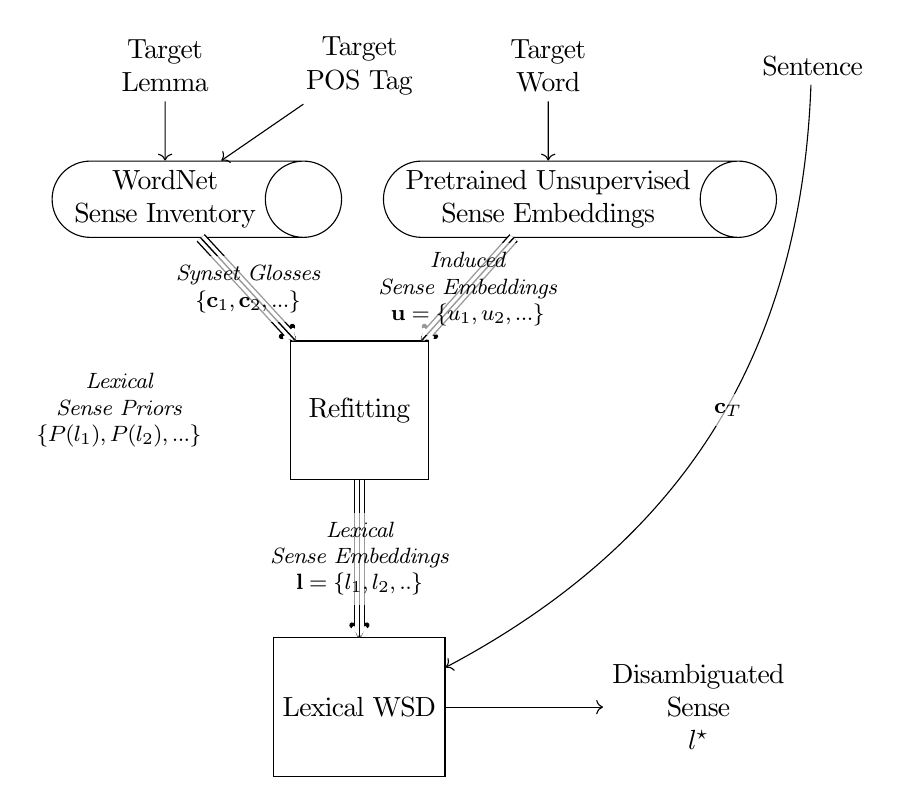
\begin{tikzpicture}[align=center]

\node[input](lemma){Target\\Lemma};
\node[input, right = 1\xunit of lemma](POS){Target\\POS Tag};
\node[input, right = 1\xunit of POS](word){Target\\ Word};
\node[datastore, below=0.75 of lemma](wordnet){WordNet \\Sense Inventory};

\node[datastore, below=0.75 of word](embeddings) {Pretrained Unsupervised \\ Sense Embeddings};
\node[proc, below=3 of POS] (refitting) {Refitting};

\node[proc, below = 2 of refitting] (WSD) {Lexical WSD};
\node[input, right = 2\xunit of word] (sentence) {Sentence};

\node[input, right = 2\xunit of WSD] (output){Disambiguated\\ Sense\\ $l^\star$};


\draw[link] (lemma) edge (wordnet);
\draw[link] (POS) edge (wordnet);
\draw[link] (word) edge (embeddings);

\draw[multi] (wordnet) -> (refitting) node[midway, labe]{Synset Glosses \\ $\{\c_1,\c_2,...\}$};
\draw[multi] (embeddings) -> (refitting) node[midway, labe]{Induced \\ Sense Embeddings \\$\u=\{u_1,u_2,...\}$};;

\draw[multi] (refitting) -> (WSD) node[midway, labe]{Lexical\\ Sense Embeddings\\ $\l=\{l_1,l_2,..\}$};
\draw[link] (sentence) edge[bend left] (WSD);
%\draw[multi, bend right] (wordnet) -> (WSD);
\triplearrow{arrows={-Implies}}{(wordnet) to[bend right] (WSD)};
\node[labe, left = 1\xunit of refitting] {Lexical\\Sense Priors\\$\{P(l_1), P(l_2),...\}$}; %hack cos benlines don't label right
\node[labe, right = 3.5\xunit of refitting] {$\c_T$}; %hack cos benlines don't label right

\draw[link] (WSD) -> (output);

\end{tikzpicture}
\end{document}
	\end{adjustbox}
	\caption{\pdfcomment{This figure is a placeholder} block diagram for performing WSD using refitting \label{WSDBlock}} 
\end{figure}
Once refitting has been used to create sense vectors that are matched to lexical word senses, we would like to use them to perform word sense disambiguation. This would show whether or not the refitted embeddings are capturing the lexical information. In this section we refer to the lexical word sense disambiguation problem\DIFdelbegin \DIFdel{-- }\DIFdelend \DIFaddbegin \DIFadd{, i.e. }\DIFaddend to take a word and find \DIFdelbegin \DIFdel{it's }\DIFdelend \DIFaddbegin \DIFadd{its }\DIFaddend dictionary sense; whereas the methods discussed in \DIFdelbegin \DIFdel{\mbox{%DIFAUXCMD
\Cref{eq:generalwsd} }%DIFAUXCMD
and \mbox{%DIFAUXCMD
\Cref{eq:generalwsdsmoothed} }%DIFAUXCMD
}\DIFdelend \DIFaddbegin \DIFadd{\mbox{%DIFAUXCMD
\Cref{eq:generalwsd,eq:generalwsdsmoothed} }%DIFAUXCMD
}\DIFaddend consider the more general word sense disambiguation problem, as applicable to disambiguate to lexical word senses, or induced word senses, depending on the inputs.
Our overall process must use both: first disambiguating the induced senses as part of refitting, then using the refitted sense vectors to find the most likely dictionary sense.
The overall process is shown in \Cref{WSDBlock}.

%DIF < Each sense of the word has a example sentence from the sense inventory.
First, we perform refitting, to transform the induced sense vectors, into lexical sense vectors.
We use the targeted word's lemma (i.e. base form), and part of speech (POS) tag to retrieve all possible definitions of the word (Glosses) from WordNet; there is one gloss per sense. These glosses are \DIFdelbegin \DIFdel{uses }\DIFdelend \DIFaddbegin \DIFadd{used }\DIFaddend as the example sentence to perform refitting. By applying refitting to the unsupervised senses using these example sentence, as discussed in \Cref{refitting}, we find embeddings, $\l=\{l_1,..., l_{n_l}\}$ for each of the lexical word senses. These lexical word senses are still supported by the language model, which means one can apply the general WSD method to determine the posterior probability of a word sense, given an observed context. 

When given a sentence $\c_{T}$, containing a target word to be disambiguated, 
the probability of each lexical word sense $P(l_i \mid \c_{T})$, can be found using \Cref{eq:generalwsd} (or the smoothed version \Cref{eq:generalwsdsmoothed}), over the lexically refitted sense embeddings. Then selecting the correct sense is simply selecting the most likely sense:
\begin{equation}
\begin{aligned}\label{eq:lexicalwsd}
l^\star (\l, \c_T) &= \argmax_{\forall l_i \in \l} P(l_i|\c_T) \\
&= \argmax_{\forall l_i \in \l} \frac{P(\c_T \mid l_i)P(l_i)}{\sum_{\forall l_j \in \l} P(\c_T \mid l_j)P(l_j)}
\end{aligned}
\end{equation}

\DIFdelbegin \DIFdel{It could be argued that lexical word senses are fitted using less than one example per class }%DIFDELCMD < \pdfcomment{I don't think it is good to start sentences with ``It could be argued...'' It sounds... argumentative. What is an alternative?}%%%
\DIFdel{. }\DIFdelend \DIFaddbegin \DIFadd{WordNet glosses are less than ideal examples sentences. As well as being definitions, rather than examples of use, they are shared across many words. }\DIFaddend Each lexical word sense shares its gloss with the rest of the set of synonymous \DIFdelbegin \DIFdel{(synsets) }\DIFdelend senses from different words \DIFaddbegin \DIFadd{(synsets)}\DIFaddend . Similarly as the synsets are defined per lemma (base word), the different lexeme (tenses and other variants) of a word also share the same example sentence. However, in both cases this does not mean that their refitted sense vectors are equal (though they are likely to be similar)\DIFdelbegin \DIFdel{, as they use different }\DIFdelend \DIFaddbegin \DIFadd{. When refitting the different lexemes correspond to different }\DIFaddend induced sense vectors, \DIFdelbegin \DIFdel{as the sense embedding system learns these on a per lexeme basis, as the components of the weighted sums.
}%DIFDELCMD < \pdfcomment{This last sentence is too long. I need to workout how to split it in two.}
%DIFDELCMD < %%%
\DIFdelend \DIFaddbegin \DIFadd{and these as well as the probabilities of the examples, are the contributing factors to the refitting sum. The limitations of the glosses does not prevent our refitting system from functioning.
}\DIFaddend 

\subsection{Lexical Sense Prior}
WordNet includes frequency counts for each word sense based on Semcor \textcite{tengi1998design}. These form a prior for $P(l_i)$.

However, Semcor is not an immense corpus, being only a subset of the Brown corpus. The comparatively small size of Semcor means that many word senses do not occur at all. As counted by WordNet 2.1, there are counts for just  36,973 word senses, out of \DIFdelbegin \DIFdel{the }\DIFdelend \DIFaddbegin \DIFadd{a }\DIFaddend total 207,016 senses in WordNet; i.e. 82\% of all senses have no count information.

An additional issue is that Semcor's underling texts from Brown are now significantly ageing. They are all from 1961 \cite{francis1979brown} -- it is not unreasonable to suggest that the frequency of word sense use has changed significantly in the last half century.

Never-the-less, the word count is the best prior readily available. Given the highly unbalanced distribution of sense occurrence a uniform prior would not be a reasonable approximation.
We apply add-one smoothing to find the prior, to remove any zero counts.
This is in addition to using our proposed geometric smoothing as an optional part of the general WSD.
Geometric smoothing which serves a different (but related) purpose, of decreasing the sharpness of the likelihood function -- not of removing impossibilities from the prior.

\subsection {Experimental Setup}
The WSD performance \DIFdelbegin \DIFdel{was }\DIFdelend \DIFaddbegin \DIFadd{is }\DIFaddend evaluated on the SemEval 2007 Task 7. 
WordNet 2.1, \DIFdelbegin \DIFdel{was }\DIFdelend \DIFaddbegin \DIFadd{is }\DIFaddend used as the sense inventory.
All glosses \DIFdelbegin \DIFdel{were }\DIFdelend \DIFaddbegin \DIFadd{are }\DIFaddend converted to lower case\DIFdelbegin \DIFdel{for use as }\DIFdelend \DIFaddbegin \DIFadd{, when used as as }\DIFaddend the example sentences \DIFdelbegin \DIFdel{for each lexical sense }\DIFdelend in the refitting step. 
They \DIFdelbegin \DIFdel{were }\DIFdelend \DIFaddbegin \DIFadd{are }\DIFaddend not clipped to a window around the target word, as the target word often does not occur at all in the gloss; and the glosses are already close to the correct size.

We \DIFdelbegin \DIFdel{used }\DIFdelend \DIFaddbegin \DIFadd{use }\DIFaddend the weighted mapping method of Agirre et al \parencite{agirre2006}, \DIFdelbegin \DIFdel{as discussed in \mbox{%DIFAUXCMD
\Cref{mapping}}%DIFAUXCMD
}\DIFdelend \DIFaddbegin \DIFadd{(see \mbox{%DIFAUXCMD
\Cref{mapping}}%DIFAUXCMD
) }\DIFaddend as a baseline \DIFdelbegin \DIFdel{; to compare an }\DIFdelend alternative method for using WSI senses for WSD.
When estimating the sense mapping weights we used both of the all-words-annotated subcorpora (Brown1 and Brown2) of SemCor as the mapping corpus.
While \DIFdelbegin \DIFdel{evaluating the }\DIFdelend \DIFaddbegin \DIFadd{calculating the weights for the the }\DIFaddend map, we do clip to a 10 word context window for each \DIFaddbegin \DIFadd{target }\DIFaddend word to be disambiguated.

The second baseline we use is the Most Frequent Sense (MFS). This method \DIFdelbegin \DIFdel{simply }\DIFdelend always disambiguates any word as having \DIFdelbegin \DIFdel{it's it's }\DIFdelend \DIFaddbegin \DIFadd{its  }\DIFaddend most common meaning. Due to the power law distribution of word senses, this is \DIFdelbegin \DIFdel{a }\DIFdelend \DIFaddbegin \DIFadd{an }\DIFaddend effective heuristic \parencite{Kilgarriff2004}.

\DIFdelbegin \DIFdel{For the }\DIFdelend \DIFaddbegin \DIFadd{We also evaluated the performance of the }\DIFaddend mapping baseline, and the Greedy embedding method, \DIFdelbegin \DIFdel{also evaluated there results }\DIFdelend with a backoff to the MSF. When a method is unable to determine the word sense, the method can report the MFS instead of returning no result (a non-attempt). For embedding methods, this occurs when a polysemous word has only one (or zero) sense embeddings trained. For the mapping method it occurs when the word does not occur in the mapping corpus. We do not report the results for AdaGram with MSF backoff, as it was trained with a \DIFdelbegin \DIFdel{high-enough }\DIFdelend \DIFaddbegin \DIFadd{large enough }\DIFaddend vocabulary, that it has almost complete coverage.

\subsection{Word Sense Disambiguation Results} \label{WSDtask}
\pgfplotstableset{
	nhundred/.style={
 		numeric type,
		precision=3,
		fixed zerofill=true,
		column type=r
%		preproc/expr={100*##1}
	}
}
\begin{table}
	\begin{adjustbox}{max width=\columnwidth}
		\DIFdelbeginFL %DIFDELCMD < \pgfplotstabletypeset[col sep=comma, header=has colnames, string type,
%DIFDELCMD < %
%DIFDELCMD < 		columns/Method/.style={ 
%DIFDELCMD < 			column type=l
%DIFDELCMD < 		},
%DIFDELCMD < %
%DIFDELCMD < 		columns/Attempted/.style={ 
%DIFDELCMD < 			column type=r
%DIFDELCMD < 		},
%DIFDELCMD < %
%DIFDELCMD < 		columns/F1/.style={nhundred},
%DIFDELCMD < 		columns/Precision/.style={nhundred},
%DIFDELCMD < 		columns/Recall/.style={nhundred},
%DIFDELCMD < %
%DIFDELCMD < 		every row 0 column F1/.style={
%DIFDELCMD < 			postproc cell content/.style={
%DIFDELCMD < 				@cell content/.add={$\bf}{$}
%DIFDELCMD < 			}
%DIFDELCMD < 		}
%DIFDELCMD < %				
%DIFDELCMD < 		]{semeval2007t7-short.csv}
%DIFDELCMD < 	%%%
\DIFdelendFL \DIFaddbeginFL \pgfplotstabletypeset[col sep=comma, header=has colnames, string type,
		every head row/.style={after row = {\toprule}},
%
		columns/Method/.style={ 
			column type=l
		},
%
		columns/Attempted/.style={ 
			column type=r
		},
%
		columns/F1/.style={nhundred},
		columns/Precision/.style={nhundred},
		columns/Recall/.style={nhundred},
%
		every row 0 column F1/.style={
			postproc cell content/.style={
				@cell content/.add={$\bf}{$}
			}
		}
%				
		]{semeval2007t7-short.csv}
	\DIFaddendFL \end{adjustbox}

	\caption{Results on SemEval 2007 Task 7 -- course-all-words disambiguation.
	The \DIFdelbeginFL \DIFdelFL{Refitted-S method denotes }\DIFdelendFL \DIFaddbeginFL \emph{\DIFaddFL{-S}} \DIFaddFL{marks results }\DIFaddendFL using \DIFdelbeginFL \DIFdelFL{refitting with }\DIFdelendFL geometric smoothing\DIFdelbeginFL \DIFdelFL{, the plain Refitted method }\DIFdelendFL \DIFaddbeginFL \DIFaddFL{.
	The }\emph{\DIFaddFL{\textasteriskcentered }} \DIFaddFL{marks }\DIFaddendFL results \DIFdelbeginFL \DIFdelFL{are without the smoothing}\DIFdelendFL \DIFaddbeginFL \DIFaddFL{with MSF backoff}\DIFaddendFL .
	} \label{samevalres}
\end{table}

The results of employing our method for WSD , are shown in \Cref{samevalres}. Our results with AdaGram when using refitting with geometric smoothing, \DIFdelbegin \DIFdel{output perform }\DIFdelend \DIFaddbegin \DIFadd{outperform }\DIFaddend the MSF baseline -- noted as a surprisingly hard baseline to beat \parencite{Chen2014}. Our results with the Greedy Embeddings, when using MSF backoff also exceed this baseline.

We found that the mapping method \parencite{agirre2006}  was not up to the task of mapping unsupervised senses to supervised senses, on this large scale task. There is simply not enough data in SemCor to allow it to properly estimate the mapping weights. The Refitting method worked significantly better. Though refitting is only usable for language model based sense embeddings, \DIFdelbegin \DIFdel{where as }\DIFdelend \DIFaddbegin \DIFadd{whereas }\DIFaddend the mapping method is suitable for all WSI systems.

While not directly comparable due to the difference in training data, we note that our Refitted results, are similar in performance, as measured by F1 score, to the results reported by Chen et al \parencite{Chen2014}.
AdaGram with smoothing, and Greedy embeddings with backoff have close to the same result as reported for L2R with backoff -- with the AdaGram slightly better and the Greedy embeddings slightly worse. They are exceeded by the best method reported in that paper: S2C method with backoff.

Our results are not strong enough for Refitted AdaGram to be used as a WSD method on its own, but \DIFdelbegin \DIFdel{the }\DIFdelend do demonstrate that the senses found by refitting are capturing the information from lexical senses.  \DIFdelbegin \DIFdel{We have demonstrated that it is now }\DIFdelend \DIFaddbegin \DIFadd{It is now evident that the refitted sense embeddings are }\DIFaddend able to perform WSD, which was not possible with the unsupervised senses. 

\section{Conclusion}\label{conclusion}

\DIFdelbegin \DIFdel{We have presented a new method }\DIFdelend \DIFaddbegin \DIFadd{A new method is proposed }\DIFaddend for taking unsupervised word embeddings, and adapting them to align to particular given \DIFdelbegin \DIFdel{uses}\DIFdelend \DIFaddbegin \DIFadd{lexical senses, or user provided usage examples}\DIFaddend . This refitting method thus allows us to find word sense embeddings with known meaning. This method can be seen as a one shot learning task, where only a single labelled example of each class is available for training.

We showed how our method could be used to create embeddings to evaluate the similarity of words, given their contexts. This in itself is a new similarity measuring method, RefittedSim\DIFdelbegin \DIFdel{, its }\DIFdelend \DIFaddbegin \DIFadd{.  RefittedSim has }\DIFaddend time complexity is $O(n \times n^\prime)$ less than that of AvgSimC. The performance of RefittedSim on AdaGrams is comparable to the results reported by the \DIFdelbegin \DIFdel{proposers }\DIFdelend \DIFaddbegin \DIFadd{researchers }\DIFaddend of other sense embeddings techniques using AvgSimC.

We also demonstrated how similar refitting principles could be used to create a set of vectors that are aligned to the meanings in a sense inventory, such as WordNet. We showed how this could be used for word sense disambiguation. On this difficult task, it performed marginally better than the \DIFaddbegin \DIFadd{hard to beat }\DIFaddend MFS baseline, and significantly better than a general mapping method used for working with WSI senses with lexical WSD tasks,

As part of our method for refitting the sense embeddings to their new senses, we presented a geometric smoothing \DIFdelbegin \DIFdel{to avoid overly certain decisions }\DIFdelend \DIFaddbegin \DIFadd{overcome the issues presented by the overly dominant senses probabilities estimates }\DIFaddend caused by limited training data.
We show that this improves the results for the similarity task with both RefittedSim, and with AvgSimC; and also \DIFdelbegin \DIFdel{that it }\DIFdelend improves the WSD results.

Our refitting method \DIFdelbegin \DIFdel{allows }\DIFdelend \DIFaddbegin \DIFadd{provided effective }\DIFaddend bridging between the vector space representation of meaning, and the traditional discrete lexical representation. More generally it allows a sense embedding to be created to model the meaning a word in any given sentence. \DIFaddbegin \DIFadd{Significant applications  of sense embeddings in tasks such as more accurate information retrieval thus become possible.
}\DIFaddend 




\newpage
\DIFaddbegin \microtypesetup{protrusion=false}
\DIFaddend \printbibliography
\DIFaddbegin 

 \DIFaddend\end{document}
